\section{Geometri Kurva Eliptik}
\label{sec:geometri-ec}

Kurva eliptik bukanlah elips. Nama itu warisan sejarah: kurva ini muncul
pertama kali ketika para matematikawan abad kesembilan belas menghitung
panjang busur sebuah elips, dan integral yang mereka hadapi ternyata mengambil
bentuk yang sama dengan integral yang mendefinisikan kurva-kurva ini. Nama itu
melekat, meskipun bentuk kurvanya sama sekali lain \citep{washington2008}.
Sebagai perkakas kriptografi, kurva ini jauh lebih muda: baru pada pertengahan
dasawarsa 1980-an Victor Miller dan Neal Koblitz mengusulkannya secara
terpisah sebagai dasar sistem kunci publik \citep{miller1986,koblitz1987}.

Yang membuat kurva eliptik menarik bagi kriptografi bukan bentuknya, melainkan
kenyataan bahwa titik-titiknya dapat ``dijumlahkan'' dengan aturan geometris
yang sederhana. Aturan itu mula-mula dirumuskan untuk kurva di atas bilangan
riil, tempat gambar dapat menolong pemahaman. Bagian ini membangun aturan
tersebut langkah demi langkah: mulai dari bentuk persamaan dan syarat
kesehatannya, lalu aturan penjumlahan dan penggandaannya, sampai akhirnya
diperlihatkan bahwa himpunan titik itu benar-benar membentuk grup abelian.

\subsection{Bentuk Weierstrass dan Syarat Ketak-singularan}
\label{subsec:weierstrass}

Kurva eliptik yang dipakai dalam kriptografi umumnya ditulis dalam bentuk
\textbf{Weierstrass}:

\begin{equation}
y^2 = x^3 + ax + b .
\label{eq:weierstrass}
\end{equation}

Setiap pasangan nilai $a$ dan $b$ menghasilkan kurva yang berbeda. Namun tidak
semua pasangan nilai boleh dipakai. Kurva eliptik disyaratkan \emph{licin}
(\textit{non-singular}), dan syaratnya adalah

\begin{equation}
4a^3 + 27b^2 \neq 0 .
\label{eq:diskriminan}
\end{equation}

Ungkapan $4a^3 + 27b^2$ itu tidak lain adalah negatif dari diskriminan polinom
kubik $x^3 + ax + b$, dan namanya menjelaskan mengapa ia penting. Bila
$4a^3 + 27b^2 = 0$, polinom kubiknya memiliki akar kembar, dan kurva yang
dihasilkan memiliki titik \textbf{singular}: titik yang tajam (\textit{cusp})
atau titik yang memotong dirinya sendiri (\textit{node}). Pada titik semacam
itu garis singgungnya tidak tunggal, sehingga aturan penjumlahan titik --- yang
seluruhnya bertumpu pada gagasan ``garis singgung di titik $P$'' --- kehilangan
makna. Tanpa aturan penjumlahan, tidak ada grup, dan tanpa grup tidak ada
kriptografi. Karena itu syarat ketak-singularan pada
Persamaan~\eqref{eq:diskriminan} diperiksa lebih dahulu sebelum sebuah kurva
dipakai \citep{hankerson2004}.

Sebagai contoh, kurva $y^2 = x^3 - 4x$ memiliki $a = -4$ dan $b = 0$, sehingga
$4(-4)^3 + 27(0)^2 = -256 \neq 0$; kurva itu licin. Persamaan ruas kanannya
dapat difaktorkan,
\[
y^2 = x^3 - 4x = x(x - 2)(x + 2),
\]
dan bentuk itu langsung memperlihatkan bahwa kurva memotong sumbu-$x$ di tiga
titik berbeda, yaitu $x = -2$, $x = 0$, dan $x = 2$. Tiga perpotongan berbeda
dengan sumbu-$x$ adalah tanda kurva yang licin. Sebaliknya, bila akarnya
kembar, dua perpotongan itu berimpit dan di situlah letak titik singularnya.

\subsection{Galeri Kurva Eliptik}
\label{subsec:galeri-kurva}

Gambar~\ref{fig:galeri-kurva} memperlihatkan lima kurva eliptik dengan
persamaan yang berbeda. Dua hal tampak sekaligus dari kumpulan gambar itu.

\begin{figure}[htbp]
    \centering
    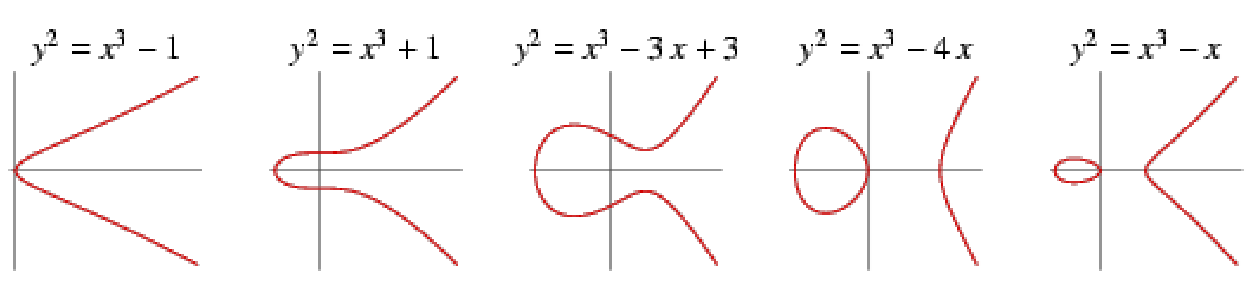
\includegraphics[width=\linewidth, height=0.32\textheight, keepaspectratio]{figures/galeri-kurva.png}
    \caption{Lima kurva eliptik dengan parameter yang berbeda: dari kiri atas
    ke kanan bawah $y^2 = x^3 - 1$, $y^2 = x^3 + 1$, $y^2 = x^3 - 3x + 3$,
    $y^2 = x^3 - 4x$, dan $y^2 = x^3 - x$. Jumlah cabang dan bentuk lengkungannya
    berubah mengikuti tanda $a$ dan $b$, tetapi sumbu simetrinya selalu sumbu-$x$}
    \label{fig:galeri-kurva}
    \sumber{Debdeep Mukhopadhyay, \textit{Elliptic Curve Cryptography}, Departemen
    Ilmu Komputer dan Teknik, IIT Madras.}
\end{figure}

Pertama, semua kurva itu simetris terhadap sumbu-$x$. Sifat itu bukan
kebetulan, melainkan akibat langsung dari Persamaan~\eqref{eq:weierstrass}:
ruas kanannya hanya bergantung pada $x$, sehingga bila titik $(x, y)$ berada
pada kurva, maka $(x, -y)$ juga. Simetri inilah yang menyediakan operasi
invers di dalam grup: lawan dari sebuah titik diperoleh dengan mencerminkannya
terhadap sumbu-$x$, tanpa perlu perhitungan apa pun.

Kedua, kurva $y^2 = x^3 - 4x$ dan $y^2 = x^3 - x$ terpisah menjadi dua bagian:
sebuah lengkungan tertutup di sebelah kiri yang menyerupai oval, dan sebuah
cabang terbuka di sebelah kanan. Yang tertutup terjadi ketika polinom kubiknya
memiliki tiga akar riil (yakni ketika $4a^3 + 27b^2 < 0$); yang terbuka terjadi
ketika hanya ada satu akar riil ($4a^3 + 27b^2 > 0$). Perbedaan bentuk itu tidak
mengubah aturan penjumlahannya sedikit pun, tetapi ia menjelaskan mengapa
kriptografi lebih suka bekerja dengan kurva yang punya satu akar riil saja:
seluruh titiknya berada pada satu cabang yang tidak terputus.

\subsection{Titik di Ketakhinggaan sebagai Elemen Netral}
\label{subsec:titik-ketakhinggaan}

Grup memerlukan elemen netral, tetapi tidak satu pun titik pada kurva memenuhi
syarat itu. Titik mana pun yang dijumlahkan dengan titik lain pasti menghasilkan
titik ketiga yang berbeda. Karena itu didefinisikan sebuah titik tambahan yang
tidak terletak pada kurva, dinamai \textbf{titik di ketakhinggaan} dan ditulis
$\mathcal{O}$. Namanya berasal dari cara kerjanya: bila dua titik yang
berlawanan, yaitu $P(x, y)$ dan $-P(x, -y)$, dihubungkan, garisnya tegak lurus
dan tidak pernah memotong kurva untuk ketiga kalinya. Dikatakan bahwa garis itu
memotong kurva ``di titik tak hingga''.

Titik itu memainkan dua peran sekaligus:

\begin{equation}
P + \mathcal{O} = \mathcal{O} + P = P ,
\qquad
P + (-P) = \mathcal{O} .
\label{eq:titik-o}
\end{equation}

Peran pertama menjadikannya elemen netral, seperti angka nol pada penjumlahan
biasa. Peran kedua menjadikannya hasil dari penjumlahan dua titik yang saling
berlawanan. Perhatikan bahwa himpunan titik pada kurva kini bertambah satu
anggota, dan tanpa anggota tambahan itu himpunan tersebut tidak akan pernah
menjadi grup.

Lawan dari sebuah titik diperoleh dengan pencerminan sederhana:
\[
\text{bila } R = (x, y) \text{ maka } -R = (x, -y) .
\]
Pada kurva di atas medan berhingga $GF(p)$, pencerminan itu diikuti
pengambilan modulo: $-R = (x, (-y) \bmod p)$. Perhatikan bahwa $(-1) \bmod 11$
sama dengan $10$, bukan $-1$; seluruh koordinat harus tetap berada di dalam
himpunan $\{0, 1, \dots, p-1\}$.

\subsection{Penjumlahan Titik Secara Geometris}
\label{subsec:penjumlahan-geometri}

Aturan penjumlahan dua titik berbeda, $P + Q = R$, dijelaskan dalam empat
langkah.

\begin{enumerate}
    \item Tarik garis lurus yang melalui $P$ dan $Q$.
    \item Bila $P \neq Q$, garis itu memotong kurva di sebuah titik ketiga;
          sebut titik itu $-R$.
    \item Cerminkan $-R$ terhadap sumbu-$x$.
    \item Pencerminan itu adalah titik $R$, yakni hasil dari $P + Q$.
\end{enumerate}

Gambar~\ref{fig:penjumlahan-titik} memperlihatkan keempat langkah itu pada
kurva $y^2 = x^3 - 3x + 3$. Garis merah melintasi $P$ dan $Q$, memotong kurva
kembali di titik $-R$, dan garis putus-putus tegak memperlihatkan pencerminan
yang menghasilkan $R$.

% Penjumlahan titik pada kurva eliptik y^2 = x^3 - 3x + 3.
% Dirujuk dari section-02.tex dengan % Penjumlahan titik pada kurva eliptik y^2 = x^3 - 3x + 3.
% Dirujuk dari section-02.tex dengan % Penjumlahan titik pada kurva eliptik y^2 = x^3 - 3x + 3.
% Dirujuk dari section-02.tex dengan \input{figures/penjumlahan-titik}.
\begin{figure}[htbp]
    \centering
    \begin{tikzpicture}[scale=1.25, >=Latex]
        % Kurva y^2 = x^3 - 3x + 3 (dua cabang: y positif dan y negatif)
        \draw[domain=-2.08:2.1, samples=200, smooth, thick, blue!70]
            plot (\x, {sqrt(\x*\x*\x - 3*\x + 3)});
        \draw[domain=-2.08:2.1, samples=200, smooth, thick, blue!70]
            plot (\x, {-sqrt(\x*\x*\x - 3*\x + 3)});

        % Sumbu koordinat
        \draw[->, gray] (-2.6,0) -- (2.6,0) node[right, font=\scriptsize] {$x$};
        \draw[->, gray] (0,-2.7) -- (0,2.7) node[above, font=\scriptsize] {$y$};

        % Garis lurus melalui P dan Q (memotong kurva untuk ketiga kalinya di -R)
        \draw[thick, red!70] (-2.0,2.237) -- (1.4,0.835);

        % Titik-titik penting
        \fill (-1.5,2.031) circle (2pt) node[above left, font=\scriptsize] {$P$};
        \fill (1,1) circle (2pt) node[right, font=\scriptsize] {$Q$};
        \fill (0.6697,1.1361) circle (2pt) node[above left, font=\scriptsize] {$-R$};
        \fill (0.6697,-1.1361) circle (2pt) node[below right, font=\scriptsize] {$R = P + Q$};

        % Pencerminan -R terhadap sumbu-x menghasilkan R
        \draw[dashed, gray] (0.6697,1.1361) -- (0.6697,-1.1361);
    \end{tikzpicture}
    \caption{Penjumlahan dua titik pada kurva eliptik $y^2 = x^3 - 3x + 3$: garis melalui $P$ dan $Q$ memotong kurva di $-R$, lalu hasilnya $R$ adalah pencerminan $-R$ terhadap sumbu-$x$}
    \label{fig:penjumlahan-titik}
\end{figure}
.
\begin{figure}[htbp]
    \centering
    \begin{tikzpicture}[scale=1.25, >=Latex]
        % Kurva y^2 = x^3 - 3x + 3 (dua cabang: y positif dan y negatif)
        \draw[domain=-2.08:2.1, samples=200, smooth, thick, blue!70]
            plot (\x, {sqrt(\x*\x*\x - 3*\x + 3)});
        \draw[domain=-2.08:2.1, samples=200, smooth, thick, blue!70]
            plot (\x, {-sqrt(\x*\x*\x - 3*\x + 3)});

        % Sumbu koordinat
        \draw[->, gray] (-2.6,0) -- (2.6,0) node[right, font=\scriptsize] {$x$};
        \draw[->, gray] (0,-2.7) -- (0,2.7) node[above, font=\scriptsize] {$y$};

        % Garis lurus melalui P dan Q (memotong kurva untuk ketiga kalinya di -R)
        \draw[thick, red!70] (-2.0,2.237) -- (1.4,0.835);

        % Titik-titik penting
        \fill (-1.5,2.031) circle (2pt) node[above left, font=\scriptsize] {$P$};
        \fill (1,1) circle (2pt) node[right, font=\scriptsize] {$Q$};
        \fill (0.6697,1.1361) circle (2pt) node[above left, font=\scriptsize] {$-R$};
        \fill (0.6697,-1.1361) circle (2pt) node[below right, font=\scriptsize] {$R = P + Q$};

        % Pencerminan -R terhadap sumbu-x menghasilkan R
        \draw[dashed, gray] (0.6697,1.1361) -- (0.6697,-1.1361);
    \end{tikzpicture}
    \caption{Penjumlahan dua titik pada kurva eliptik $y^2 = x^3 - 3x + 3$: garis melalui $P$ dan $Q$ memotong kurva di $-R$, lalu hasilnya $R$ adalah pencerminan $-R$ terhadap sumbu-$x$}
    \label{fig:penjumlahan-titik}
\end{figure}
.
\begin{figure}[htbp]
    \centering
    \begin{tikzpicture}[scale=1.25, >=Latex]
        % Kurva y^2 = x^3 - 3x + 3 (dua cabang: y positif dan y negatif)
        \draw[domain=-2.08:2.1, samples=200, smooth, thick, blue!70]
            plot (\x, {sqrt(\x*\x*\x - 3*\x + 3)});
        \draw[domain=-2.08:2.1, samples=200, smooth, thick, blue!70]
            plot (\x, {-sqrt(\x*\x*\x - 3*\x + 3)});

        % Sumbu koordinat
        \draw[->, gray] (-2.6,0) -- (2.6,0) node[right, font=\scriptsize] {$x$};
        \draw[->, gray] (0,-2.7) -- (0,2.7) node[above, font=\scriptsize] {$y$};

        % Garis lurus melalui P dan Q (memotong kurva untuk ketiga kalinya di -R)
        \draw[thick, red!70] (-2.0,2.237) -- (1.4,0.835);

        % Titik-titik penting
        \fill (-1.5,2.031) circle (2pt) node[above left, font=\scriptsize] {$P$};
        \fill (1,1) circle (2pt) node[right, font=\scriptsize] {$Q$};
        \fill (0.6697,1.1361) circle (2pt) node[above left, font=\scriptsize] {$-R$};
        \fill (0.6697,-1.1361) circle (2pt) node[below right, font=\scriptsize] {$R = P + Q$};

        % Pencerminan -R terhadap sumbu-x menghasilkan R
        \draw[dashed, gray] (0.6697,1.1361) -- (0.6697,-1.1361);
    \end{tikzpicture}
    \caption{Penjumlahan dua titik pada kurva eliptik $y^2 = x^3 - 3x + 3$: garis melalui $P$ dan $Q$ memotong kurva di $-R$, lalu hasilnya $R$ adalah pencerminan $-R$ terhadap sumbu-$x$}
    \label{fig:penjumlahan-titik}
\end{figure}


Perlu diperhatikan bahwa langkah pencerminan bukan hiasan. Bila ia dihilangkan,
aturan penjumlahan itu tidak akan bersifat asosiatif, dan himpunan titiknya
tidak akan membentuk grup. Pencerminan itulah yang mengubah hubungan geometris
sederhana ``tiga titik segaris'' menjadi operasi aljabar yang taat hukum.

\subsection{Penurunan Analitik Rumus Penjumlahan}
\label{subsec:analitik-penjumlahan}

Penjelasan geometris di atas cukup untuk memahami mengapa aturan itu masuk
akal, tetapi implementasinya menuntut rumus yang dapat dihitung. Rumus itu
diturunkan dengan mensubstitusikan persamaan garis ke persamaan kurva.

Misalkan garis $g$ melalui $P(x_p, y_p)$ dan $Q(x_q, y_q)$ ditulis
$y = mx + c$, dengan gradien

\begin{equation}
m = \frac{y_q - y_p}{x_q - x_p} \qquad (\text{untuk } P \neq Q).
\label{eq:gradien-pq}
\end{equation}

Perpotongan garis $g$ dengan kurva $y^2 = x^3 + ax + b$ terjadi ketika
$(mx + c)^2 = x^3 + ax + b$, yaitu ketika

\[
x^3 - m^2x^2 + (a - 2mc)x + (b - c^2) = 0 .
\]

Persamaan itu berderajat tiga, sehingga tepat memiliki tiga akar. Ketiga akar
itu adalah absis dari ketiga titik potongnya, yaitu $x_p$, $x_q$, dan $x_r$
(jadi $x_r$ adalah absis dari $-R$, yang nanti dicerminkan). Menurut hubungan
Vieta, jumlah ketiga akar sebuah polinom kubik $x^3 + \alpha x^2 + \beta x +
\gamma$ sama dengan $-\alpha$. Karena koefisien $x^2$ di sini adalah $-m^2$,
diperoleh

\[
x_p + x_q + x_r = m^2 ,
\]

sehingga

\begin{equation}
\begin{aligned}
x_r &= m^2 - x_p - x_q \pmod{p}, \\
y_r &= m(x_p - x_r) - y_p \pmod{p} .
\end{aligned}
\label{eq:koordinat-pq}
\end{equation}

Rumus kedua pada Persamaan~\eqref{eq:koordinat-pq} berasal dari kenyataan bahwa
$\pm R$ terletak pada garis yang sama dengan $P$ dan $Q$. Karena $y = mx + c$
dan $c = y_p - mx_p$, ordinat titik $-R$ adalah $mx_r + c$; mencerminkannya
terhadap sumbu-$x$ mengubah tandanya, sehingga
\[
y_r = -(mx_r + y_p - mx_p) = m(x_p - x_r) - y_p .
\]

Sebagai contoh, ambil kurva $y^2 = x^3 + 2x + 4$ beserta titik $P(2, 4)$ dan
$Q(0, 2)$. Keduanya memang berada pada kurva, sebab $4^2 = 8 + 4 + 4 = 16$ dan
$2^2 = 0 + 0 + 4 = 4$. Dengan Persamaan~\eqref{eq:gradien-pq} diperoleh
\[
m = \frac{2 - 4}{0 - 2} = \frac{-2}{-2} = 1 ,
\]
lalu dengan Persamaan~\eqref{eq:koordinat-pq}
\[
x_r = 1^2 - 2 - 0 = -1,
\qquad
y_r = 1 \cdot (2 - (-1)) - 4 = 3 - 4 = -1 .
\]
Jadi $R(-1, -1)$. Pemeriksaannya: $(-1)^2 = 1$ dan
$(-1)^3 + 2(-1) + 4 = -1 - 2 + 4 = 1$. Cocok, sehingga $R$ benar-benar titik
pada kurva.

Berkas sumber menuliskan gradien sebagai $m = (y_p - y_q)/(x_p - x_q)$,
sedangkan Persamaan~\eqref{eq:gradien-pq} memakai bentuk yang lazim ditulis di
buku rujukan, yaitu $m = (y_q - y_p)/(x_q - x_p)$. Keduanya memberi nilai yang
sama, sebab menukar tanda pembilang dan penyebut tidak mengubah hasil
baginya. Perlu diperhatikan pula bahwa pada medan berhingga pembagian
digantikan perkalian dengan invers modulo, sehingga

\begin{equation}
m \equiv (y_q - y_p)(x_q - x_p)^{-1} \pmod{p} .
\label{eq:gradien-mod-p}
\end{equation}

\subsection{Penggandaan Titik}
\label{subsec:penggandaan-titik}

Penjumlahan dua titik berbeda belum cukup untuk menghitung perkalian skalar.
Perkalian $3P$ misalnya menuntut penjumlahan $P$ dengan dirinya sendiri, dan
pada kasus itu garis yang melalui kedua titiknya bukan lagi garis potong
biasa, melainkan \textbf{garis singgung} di $P$. Operasi inilah yang disebut
\textbf{penggandaan titik} (\textit{point doubling}) dan ditulis
$P + P = 2P = R$.

Karena gradien garis singgung adalah turunan kurva di titik tersebut, nilai
$m$ diperoleh dengan menurunkan Persamaan~\eqref{eq:weierstrass} secara
implisit. Dari $2y \frac{dy}{dx} = 3x^2 + a$ diperoleh

\begin{equation}
m = \frac{dy}{dx} = \frac{3x_p^2 + a}{2y_p} ,
\label{eq:gradien-penggandaan}
\end{equation}

sehingga koordinat hasilnya

\begin{equation}
\begin{aligned}
x_r &= m^2 - 2x_p \pmod{p}, \\
y_r &= m(x_p - x_r) - y_p \pmod{p} .
\end{aligned}
\label{eq:koordinat-penggandaan}
\end{equation}

Secara aljabar, rumus itu tetap merupakan penerapan hubungan Vieta. Pada
kasus penggandaan, garis singgung menyentuh kurva di $P$, sehingga akar $x_p$
muncul dua kali: $x_p + x_p + x_r = m^2$, dan karena itu
$x_r = m^2 - 2x_p$. Gambar~\ref{fig:penggandaan-titik} memperlihatkan
geometrinya.

\begin{figure}[htbp]
    \centering
    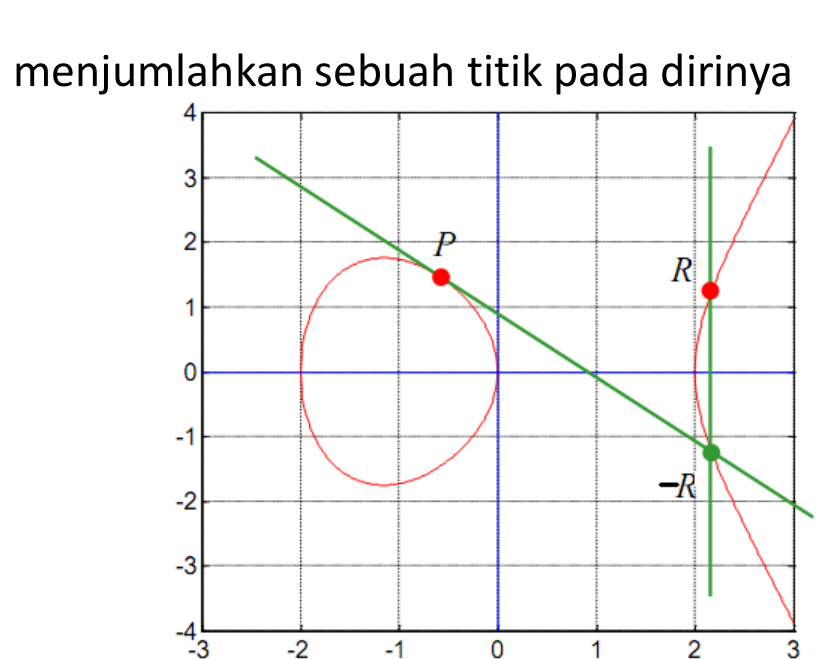
\includegraphics[width=0.6\linewidth, height=0.5\textheight, keepaspectratio]{figures/penggandaan-titik.png}
    \caption{Penggandaan titik pada kurva eliptik: garis singgung di titik $P$
    memotong kurva di $R$, dan pencerminan $R$ terhadap sumbu-$x$ menghasilkan
    $2P$}
    \label{fig:penggandaan-titik}
    \sumber{Munir, \textit{IF4020 Kriptografi}, ITB.}
\end{figure}

Satu keadaan khusus perlu diperhatikan. Bila ordinat titik $P$ sama dengan
nol, yaitu $y_p = 0$, maka Persamaan~\eqref{eq:gradien-penggandaan} membagi
dengan nol dan $m$ tidak terdefinisi. Secara geometris, garis singgung di titik
itu tegak lurus, sehingga tidak pernah menyentuh kurva untuk kedua kalinya.
Dalam keadaan itu
\[
P + P = 2P = \mathcal{O} .
\]
Titik-titik berordinat nol pada kurva licin justru adalah akar-akar polinom
kubik $x^3 + ax + b$; pada kurva $y^2 = x^3 - 4x$ misalnya, ketiga titik
$(-2, 0)$, $(0, 0)$, dan $(2, 0)$ masing-masing berorde dua di dalam grup.

Sebagai contoh penerapan, ambil kembali $P(2, 4)$ pada $y^2 = x^3 + 2x + 4$.
Dengan $a = 2$,
\[
m = \frac{3(2)^2 + 2}{2(4)} = \frac{14}{8} = \frac{7}{4},
\]
sehingga
\[
x_r = \left(\frac{7}{4}\right)^2 - 2(2) = \frac{49}{16} - 4 = -\frac{15}{16},
\qquad
y_r = \frac{7}{4}\left(2 + \frac{15}{16}\right) - 4 = \frac{73}{64} .
\]
Jadi $2P = \left(-\frac{15}{16}, \frac{73}{64}\right)$, atau dalam pecahan
desimal $(-0{,}9375;\ 1{,}140625)$. Angka pecahan itu sekaligus menunjukkan
mengapa kurva di atas bilangan riil tidak dipakai untuk kriptografi: koordinat
titiknya cepat berubah menjadi pecahan yang panjang, dan penyimpanannya di dalam
komputer menuntut pembulatan yang hasilnya tidak lagi dapat dipercaya.

\subsection{Pelelaran Titik dan Perkalian Skalar}
\label{subsec:pelelaran-titik}

Dengan penjumlahan dan penggandaan di tangan, sebuah titik dapat dijumlahkan
dengan dirinya sendiri berkali-kali. Operasi itu disebut \textbf{pelelaran
titik} (\textit{point iteration}) atau \textbf{perkalian skalar}:

\begin{equation}
kP = \underbrace{P + P + \dots + P}_{k \text{ kali}} .
\label{eq:pelelaran}
\end{equation}

Di sini $k$ adalah skalar (bilangan bulat) sedangkan $P$ dan hasilnya adalah
titik. Untuk $k = 3$ diperoleh $3P = P + P + P$ atau, lebih hemat,
$3P = 2P + P$: cukup satu penggandaan ditambah satu penjumlahan, bukan dua
penjumlahan.

Cara menghitung $kP$ secara efisien bukanlah menjumlahkan $P$ sebanyak $k-1$
kali, melainkan memanfaatkan bentuk biner $k$ --- teknik yang dikenal sebagai
\textit{double-and-add}. Sebagai contoh, untuk $k = 23$ yang bentuk binernya
$10111_2$,
\[
23P = 2\bigl(2(2(2P) + P) + P\bigr) + P .
\]
Rangkaian itu hanya memerlukan empat penggandaan dan tiga penjumlahan, yaitu
tujuh operasi titik, bukan dua puluh dua. Secara umum, biaya menghitung $kP$
hanyalah sebanding dengan banyaknya bit $k$, yakni sekitar $\log_2 k$
penggandaan ditambah paling banyak $\log_2 k$ penjumlahan. Sifat inilah yang
membuat ECC praktis: kunci privat sepanjang 256 bit hanya menuntut sekitar
$256$ penggandaan dan $128$ penjumlahan, sekalipun skalarnya berukuran
$10^{77}$.

Algoritma \textit{double-and-add} juga menyimpan asimetri yang menjadi inti
keamanan ECC. Arah maju --- dari $k$ dan $P$ menuju $kP$ --- hanya memerlukan
operasi yang berjumlah logaritmik. Arah mundur --- dari $P$ dan $kP$ menuju $k$
--- tidak diketahui cara efisiennya. Asimetri itu dibahas pada
Bagian~\ref{sec:kriptografi-ec}.

\subsection{Kurva Eliptik Membentuk Grup Abelian}
\label{subsec:grup-eliptik}

Sekarang seluruh perkakas tersedia untuk menjawab pertanyaan yang diajukan di
awal bagian ini. Misalkan $G$ adalah himpunan semua titik $P(x, y)$ yang
memenuhi $y^2 = x^3 + ax + b$ ditambah titik di ketakhinggaan $\mathcal{O}$,
dan misalkan operasi binernya adalah aturan penjumlahan yang baru saja
diturunkan. Tabel~\ref{tab:aksioma-grup-eliptik} memeriksa kelima aksioma grup.

\begin{table}[htbp]
    \centering
    \caption{Pemeriksaan kelima aksioma grup pada $\langle G, + \rangle$}
    \label{tab:aksioma-grup-eliptik}
    \begin{tabularx}{\linewidth}{@{}l l
                                   >{\raggedright\arraybackslash}X@{}}
    \toprule
    \textbf{Aksioma} & \textbf{Pemeran} & \textbf{Alasan} \\
    \midrule
    Ketertutupan & hasil $P + Q$ &
    Rumus pada Persamaan~\eqref{eq:koordinat-pq} hanya memakai operasi medan,
    sehingga koordinat hasilnya selalu berada di dalam medan yang sama \\
    \addlinespace
    Asosiatif & --- &
    $P + (Q + R) = (P + Q) + R$; dapat dibuktikan dengan substitusi rumus,
    dan secara geometris setara dengan teorema geometri proyektif klasik \\
    \addlinespace
    Elemen netral & $\mathcal{O}$ &
    $P + \mathcal{O} = \mathcal{O} + P = P$ menurut
    Persamaan~\eqref{eq:titik-o} \\
    \addlinespace
    Elemen invers & $-P = (x_p, -y_p)$ &
    $P + (-P) = \mathcal{O}$; lawan setiap titik tersedia karena kurva
    simetris terhadap sumbu-$x$ \\
    \addlinespace
    Komutatif & --- &
    $P + Q = Q + P$; rumus gradien pada Persamaan~\eqref{eq:gradien-pq}
    simetris terhadap pertukaran $P$ dan $Q$ \\
    \bottomrule
    \end{tabularx}
\end{table}

Karena kelima aksioma terpenuhi --- termasuk yang kelima --- maka
$\langle G, + \rangle$ adalah \textbf{grup abelian}. Perhatikan bahwa
komutativitas bukan tambahan yang kebetulan berlaku, melainkan akibat dari
bentuk rumusnya: membalik urutan $P$ dan $Q$ hanya mengubah tanda pembilang dan
penyebut gradien secara bersamaan.

Satu catatan penutup perlu disampaikan mengenai orde grup. Banyaknya titik pada
sebuah kurva eliptik di atas $GF(p)$ tidak dapat ditentukan hanya dari $p$;
untuk $p = 11$ kurva $y^2 \equiv x^3 + x + 6$ memiliki $13$ elemen, sedangkan
kurva lain dengan modulus yang sama dapat memiliki jumlah yang berbeda. Dalil
Hasse membatasi jumlah itu pada selang $p + 1 - 2\sqrt{p}$ sampai
$p + 1 + 2\sqrt{p}$, tetapi nilai tepatnya harus dihitung. Bagi perancang
sistem, hal itu berarti kurva tidak boleh dipilih sembarangan: ordonya harus
diperiksa lebih dahulu, dan bagian berikutnya memperlihatkan bagaimana
pemeriksaan itu dijalankan pada kurva kecil.
